\documentclass[twocolumn,pdftex]{aastex701}
\usepackage{amsmath,amssymb}
\hypersetup{colorlinks,citecolor=blue,linkcolor=magenta,urlcolor=blue}

\newcommand{\msun}{M_{\odot}}
\newcommand{\Mh}{M_{\rm h}}
\newcommand{\mhsix}{M_{\rm h,6}}
\newcommand{\Tthree}{T_{3}}
\newcommand{\xhh}{x_{\rm H_2}}
\newcommand{\Zp}{Z'}
\newcommand{\fst}{f_{\ast}}
\newcommand{\fOm}{f_{\Omega}}
\newcommand{\Geq}{\Gamma_{\rm eq}}
\newcommand{\GL}{GL26}
\newcommand{\kms}{\,{\rm km\,s^{-1}}}
\newcommand{\Htwo}{{\rm H_2}}

\shorttitle{A Metal-Poor Tidal Disruption Engine}
\shortauthors{Guillochon and Loeb}

\begin{document}

\title{A Metal-Poor Tidal Disruption Engine: The Warm Molecular Equilibrium and Its Application to Little Red Dots}

\correspondingauthor{James Guillochon}

\author[0000-0002-9809-8215]{James Guillochon}
\affiliation{Harvard-Smithsonian Center for Astrophysics, The Institute for Theory and Computation, 60 Garden Street, Cambridge, MA 02138, USA}
\email[show]{guillochon@gmail.com}

\author[0000-0003-4330-287X]{Abraham Loeb}
\affiliation{Harvard-Smithsonian Center for Astrophysics, The Institute for Theory and Computation, 60 Garden Street, Cambridge, MA 02138, USA}
\email{aloeb@cfa.harvard.edu}

\begin{abstract}
The unbound debris of tidal disruption events can sustain a self-regulating equilibrium in galactic nuclei: momentum injected into surrounding molecular clouds compresses the nuclear star cluster until stellar collisions cap the disruption rate at $\Gamma_{\rm eq}\simeq1.4\times10^{-2}\,M_{\rm h,6}^{-0.84}\,{\rm yr^{-1}}$ (Guillochon \& Loeb 2026). That solution relies on CO and dust to hold the clouds at 10~K and does not apply to the metal-poor nuclei in which little red dots (LRDs) form. We re-derive it with ${\rm H_2}$ rotational cooling in local thermodynamic equilibrium and find that the engine survives on a warm branch. The collision cap and the belt radius do not involve cooling, so $\Gamma_{\rm eq}$, $r_{\rm b}\simeq4.9\,M_{\rm h,6}$~pc and $n_{\rm MC}\simeq1.9\times10^{5}\,M_{\rm h,6}^{-2}\,{\rm cm^{-3}}$ carry over unchanged. ${\rm H_2}$-cooled clouds have no thermostat; they are heated volumetrically by the keV emission of the radiative remnants, in the manner of X-ray dissociation regions, and their temperature is bracketed by the requirements that they fit within the disk and remain supersonically turbulent, $740\,M_{\rm h,6}^{-0.40}\lesssim T_{\rm MC}\lesssim1100\,M_{\rm h,6}^{-0.36}$~K. In this window the cloud radii, gas mass ($\sim3\times10^{5}\,M_{\odot}$) and mass floor ($\sim10^{6}\,M_{\odot}$) match the metal-rich solution to within factors of two, while the observables differ sharply: the extinction falls to $A_V\simeq27\,Z'$, and the belt dust, which responds only to the duty-cycle-averaged luminosity, reradiates $\sim1$ per cent of the flare luminosity at $\sim60$~K, removing the tension with the dust deficit of LRDs; AGN radiation pressure becomes negligible; the black hole grows mainly through disruptions; and the injected energy emerges as ${\rm H_2}$ lines with $L_{\rm H_2}\simeq8\times10^{40}\,M_{\rm h,6}^{-0.5}\,{\rm erg\,s^{-1}}$. The engine operates for $10^{6}\lesssim M_{\rm h}\lesssim(1.5$--$5)\times10^{6}\,M_{\odot}$ and $10^{-3}\lesssim Z'\lesssim0.3$, a range that contains the measured metallicities of LRD hosts, and at a duty cycle of $\sim7$ per cent above a tenth of Eddington it requires an LRD host abundance of $\sim10^{-4}$~cMpc$^{-3}$.
\end{abstract}

\keywords{Tidal disruption (1696) --- Active galactic nuclei (16) --- Supermassive black holes (1663) --- Molecular clouds (1072) --- High-redshift galaxies (734)}

\section{Introduction}\label{sec:intro}

The compact, red, broad-lined sources uncovered by JWST at $z\sim4$--9 and known as little red dots \citep[LRDs;][]{Matthee:2024a,Greene:2024a,Harikane:2023a,Kocevski:2025a} are abundant, with number densities of order $10^{-5}$--$10^{-4}$~cMpc$^{-3}$ \citep{Matthee:2024a,Kokorev:2024a,Akins:2025a}, compact, and puzzling in their spectral energy distributions, which show a marked deficit of both hot and cold dust emission \citep{Setton:2025a,Chen:2025a,Casey:2025a} alongside reddening that may arise from dense gas rather than dust \citep{Inayoshi:2025a,Naidu:2025a,deGraaff:2026a}. Their hosts are metal-poor, with direct-method oxygen abundances of $Z'\simeq0.08$ and a spread of $\sim0.6$~dex \citep{Nikopoulos:2026a}. Among the interpretations proposed for them is that they are powered by the recurrent tidal disruption of stars in nuclei that have recently built a black hole by runaway stellar collisions \citep{Bellovary:2025a,Pacucci:2025a,Kritos:2026a}; the radio-quiet character of the population is consistent with this \citep{Perger:2025a}, and the residual stellar cores left behind by seed formation are dense enough to sustain high disruption rates \citep{Pacucci:2025a}.

What that picture lacks is a mechanism that sets the disruption rate. \citet[hereafter \GL]{Guillochon:2026a} supply one. In that model the unbound debris of each disruption drives a supernova-like remnant into the molecular clouds surrounding the nucleus; the momentum keeps the clouds turbulent and dense, the dense clouds shorten the relaxation time of the nuclear star cluster, and the compressed cluster disrupts stars faster still. The runaway is arrested when stars begin to collide, and the steady state has $\Geq \simeq 1.4\times10^{-2}\,\mhsix^{-0.84}\,{\rm yr^{-1}}$, where $\mhsix \equiv \Mh/10^{6}\,\msun$. \GL\ noted (\S7.2) that the equilibrium rates and stellar densities coincide with those inferred for LRD cores, but also identified two obstacles to applying the model there. The first is obscuration: the metal-rich engine is buried under $A_V\simeq50$, whereas LRDs lack dust emission. The second is metallicity: the energy-balance condition of \GL\ uses CO line cooling with the clouds held at 10~K by the balance of cosmic-ray heating and molecular cooling, neither of which is available in gas with $Z\lesssim 0.1\,Z_\odot$. As \GL\ put it, the condition ``would have to be rederived with molecular hydrogen or atomic cooling.''

This paper carries out that re-derivation. We keep every element of the \GL\ framework---the Bahcall--Wolf cusp, the tidally marginal cloud belt, the covering, energy, collision and compression conditions, and the monomial solution method---and change only the microphysics of the cooling: the volumetric cooling rate, the sound speed of the clouds, and the radiative time of the unbound debris remnants, each of which depends on composition. The structure of the \GL\ solution turns out to isolate the effect of metallicity cleanly. Of the four unknowns describing the equilibrium, two are fixed by conditions that do not involve cooling at all, and the two that remain inherit the composition dependence in a way that can be written as exact power laws in the cloud temperature, the $\Htwo$ abundance, and the metallicity.

The paper is organized as follows. Section~\ref{sec:engine} summarizes the \GL\ equilibrium and identifies where composition enters. Section~\ref{sec:cooling} describes the cooling of metal-poor gas at the densities of interest and argues that the cold, CO-cooled branch of the equilibrium cannot exist there. Section~\ref{sec:equilibrium} solves for the warm, $\Htwo$-cooled branch and shows that the cloud temperature, which in \GL\ was an external input, is here bracketed by two internal consistency requirements. Section~\ref{sec:lrd} draws out the observable consequences for LRDs, Section~\ref{sec:caveats} discusses the limitations of the treatment, and Section~\ref{sec:summary} summarizes. Throughout, normalized quantities are indicated by a subscript, so that $\Tthree \equiv T_{\rm MC}/10^{3}$~K, $\Zp \equiv Z/Z_\odot$, and $\xhh$ is the fraction of hydrogen nuclei bound in $\Htwo$.

\section{The engine and where composition enters}\label{sec:engine}

We follow the notation of \GL, to which we refer the reader for the derivations; here we restate only what is needed to see where the cooling function appears.

The nucleus is a relaxed Bahcall--Wolf cusp, $n_\ast\propto r^{-7/4}$, containing a stellar mass $2\Mh$ within the sphere of influence $a_{\rm h} = 2G\Mh/\sigma^2$, with mean stellar mass $m_\ast = 0.5\,\msun$ and radius $R_\ast = 0.46\,R_\odot$ \citep{Tout:1996a}. The stars occupy a fraction $\fst$ of $4\pi$ steradians. Molecular clouds orbit in a belt of radius $r_{\rm b}$ and aspect ratio $\fOm = H/r_{\rm b}$, where they are marginally tidally bound,
\begin{equation}
\rho_{\rm MC} = \frac{9\Mh}{4\pi r_{\rm b}^{3}},
\label{eq:tidal}
\end{equation}
and supported against self-gravity by supersonic turbulence,
\begin{equation}
\mathcal{M}^{2}c_{\rm s}^{2} = \frac{4\pi}{5}G\rho_{\rm MC}R_{\rm MC}^{2},
\label{eq:virial}
\end{equation}
with $\sigma_{\rm cl} = \mathcal{M}c_{\rm s}$ the turbulent velocity and $\tau_{\rm c} = 2R_{\rm MC}/\sigma_{\rm cl}$ the crossing time on which the turbulence decays. The number of clouds needed to pave the belt is $N_{\rm MC} = 4\fOm r_{\rm b}^{2}/R_{\rm MC}^{2}$, and the stars are fed from the disk so that the debris is beamed back into it ($b=1$ in the notation of \GL).

Four conditions close the system. The first (\GL\ eq.~23) requires every patch of the belt to be struck by an unbound debris remnant (UDR) at least once per crossing time,
\begin{equation}
\Gamma_{\rm TDE}\,f_{\rm UDR}\,\tau_{\rm c}\,\beta = 1,\qquad f_{\rm UDR} = \frac{R_{\rm UDR}^{2}}{4r_{\rm b}^{2}},
\label{eq:C1}
\end{equation}
with $\beta = b/\fOm$ and $R_{\rm UDR}$ the radius at which a remnant of energy $E_{\rm UDR} = 1.8\times10^{50}\,\mhsix^{1/3}$~erg \citep{Guillochon:2016b} becomes radiative in gas of density $\rho_{\rm MC}$ \citep{Sedov:1946a,Taylor:1950a,Blondin:1998a}. The second (\GL\ eq.~27) requires the clouds to radiate the energy they receive,
\begin{equation}
\Gamma_{\rm TDE}\,E_{\rm UDR}\,b = L_{\rm MC} = N_{\rm MC}V_{\rm MC}\,\Lambda_{\rm vol},
\label{eq:C2}
\end{equation}
where $V_{\rm MC} = 4\pi R_{\rm MC}^{3}/3$ and $\Lambda_{\rm vol}$ is the volumetric cooling rate of the cloud gas. The third (\GL\ eq.~29) caps the disruption rate at the rate at which stars collide before reaching the loss cone,
\begin{equation}
\Gamma_{\rm coll}/\fst = \Gamma_{\rm TDE},
\label{eq:C3}
\end{equation}
where $\Gamma_{\rm coll}$ is the gravitationally focused collision rate integrated over the cusp (\GL\ eq.~30) and $\Gamma_{\rm TDE}$ is the bridged Cohn--Kulsrud loss-cone flux \citep{Cohn:1978a,Merritt:2013a,Vasiliev:2013a,Stone:2016a}. The fourth (\GL\ eq.~32) is an inequality rather than a closure: the clouds must dominate the relaxation of the cusp, $t_{\rm relax,MC} \le t_{\rm relax,\ast}$, which sets a lower bound on $\Mh$.

Composition enters in three places. The cooling rate $\Lambda_{\rm vol}$ in equation~(\ref{eq:C2}) is the most obvious; \GL\ take $\Lambda_{\rm vol} = \Lambda_0 n_{\rm MC}^{2}$ with $\Lambda_0 = 1.3\times10^{-27}$~erg~cm$^{3}$~s$^{-1}$, appropriate to CO at 10~K \citep{Goldsmith:1978a,Neufeld:1995a}. The sound speed $c_{\rm s}$ in equation~(\ref{eq:virial}) depends on the cloud temperature and mean molecular weight; \GL\ take $c_{\rm s} = 0.19\kms$ for 10~K gas at $\mu = 2.33$. And the radiative time of the remnant, $\tau_{\rm rad}$, which sets $R_{\rm UDR}$ in equation~(\ref{eq:C1}), was taken from numerical calculations at solar composition \citep{Blondin:1998a} and depends on the cooling of the hot, shocked phase. Nothing else in the system knows about metallicity. In particular, the collision condition (\ref{eq:C3}) involves only the cusp, so the equilibrium dispersion and disruption rate,
\begin{align}
\sigma_{\rm eq} &= 2.4\times10^{2}\,\mhsix^{0.03}\kms, \nonumber\\
\Geq &\simeq 1.4\times10^{-2}\left(\frac{\fst}{0.22}\right)^{2.4}\mhsix^{-0.84}\,{\rm yr^{-1}},
\label{eq:Geq}
\end{align}
are the same for any composition, as are $a_{\rm h} = 0.15\,\mhsix^{0.94}$~pc and the central density $\rho_0 = 6\times10^{7}\,\mhsix^{-1.8}\,\msun\,{\rm pc^{-3}}$ at $\fst = 0.22$. Metallicity affects the gas, not the stars.

\section{Cooling of metal-poor gas in the belt}\label{sec:cooling}

\subsection{Why the cold branch does not exist at low metallicity}\label{sec:coldbranch}

In the \GL\ solution the cloud temperature is not an output of the engine but an external thermostat: the clouds sit at $\sim10$~K because CO and dust cooling are so steep below H recombination that the gas rapidly settles where cooling balances cosmic-ray heating \citep{Krumholz:2015a}. The engine then adjusts the cloud size, count, and mass so that the CO luminosity of the belt matches the UDR power.

Both halves of that thermostat scale with metallicity. The CO abundance, and hence $\Lambda_0$, is proportional to $\Zp$ for $\Zp\lesssim1$, and the dust that thermally couples to the gas at the highest densities is likewise diluted. Reducing $\Lambda_0$ by $\Zp$ in equation~(\ref{eq:C2}) at fixed 10~K, holding the other conditions fixed, inflates the required cloud radius as $R_{\rm MC}\propto\Zp^{-1}$: the clouds outgrow the disk half-thickness $H\simeq1$~pc that is supposed to contain them for $\Zp\lesssim0.7$, and at $\Zp = 0.1$ have radii of 7~pc, so the solution fails the geometric requirement that \GL\ use to bound $\fst$ from below. Holding the gas at 10~K is in any case not permitted. The thermostat is gone with the CO and dust that set it, and at the redshifts of LRDs the cosmic microwave background alone imposes a floor of $T_{\rm CMB}=16$--22~K at $z=5$--7, so even the metal-rich comparison values of \GL\ should be read as a $\sim20$~K rather than a 10~K state there. The remaining low-temperature coolants in gas with $\Zp\lesssim0.1$ are the [C\,{\sc ii}]~158~$\mu$m and [O\,{\sc i}]~63~$\mu$m fine-structure lines, whose efficiency also scales with $\Zp$, and below a critical metallicity of order $10^{-3.5}\,Z_\odot$ they cease to be competitive with $\Htwo$ \citep{Bromm:2003a,Omukai:2000a,Santoro:2006a,Glover:2007a}. This argument does not exclude an intermediate state at $\Zp\sim0.3$--0.7 in which CO and fine-structure lines at a few tens to a few hundred K, where they radiate far more per nucleus than at 10~K, cool clouds that do fit within the disk; we return to that regime in Section~\ref{sec:xh2}. What it does establish is that there is no metal-poor analogue of the 10~K state that the \GL\ engine can occupy.

\subsection{$\Htwo$ cooling at the belt density}\label{sec:h2cool}

What metal-poor gas does have is molecular hydrogen. At the densities the equilibrium will return, $n_{\rm MC}\sim10^{5}$~cm$^{-3}$, the rotational levels of $\Htwo$ are thermalized: the critical density for the pure rotational cooling is of order $10^{3}$--$10^{4}$~cm$^{-3}$ at $T\sim10^{3}$~K for collisions with atomic hydrogen \citep{Hollenbach:1979a,Galli:1998a,Glover:2008a}, and up to $\sim10^{5}$~cm$^{-3}$ when $\Htwo$ itself is the collider \citep{LeBourlot:1999a,Coppola:2019a}, so the cooling is in the local thermodynamic equilibrium (LTE) regime and scales with the first power of density rather than the second. We adopt the LTE rotational cooling rate per molecule of \citet{Hollenbach:1979a}, which over the range $200\lesssim T\lesssim2000$~K is well represented by the single power law
\begin{equation}
L_{\rm LTE}(T) \simeq 9.5\times10^{-22}\,\Tthree^{3.76}\ {\rm erg\,s^{-1}\ per\ H_2},
\label{eq:LLTE}
\end{equation}
where we have dropped the correction factors that enter the full fit; they are 0.9 at $10^{3}$~K and 0.65 at $2\times10^{3}$~K. The volumetric cooling rate of a cloud with hydrogen-nucleus density $n_{\rm MC}$ and molecular fraction $\xhh$ is then
\begin{equation}
\Lambda_{\rm vol} = \xhh\,\frac{n_{\rm MC}}{2}\,L_{\rm LTE}(T_{\rm MC}).
\label{eq:Lvol}
\end{equation}
We take a primordial composition for the belt gas, with hydrogen mass fraction $X = 0.76$, so that $n_{\rm MC} = \rho_{\rm MC}/1.32\,m_{\rm p}$ and, for fully molecular gas, $\mu = 2.27$ and
\begin{equation}
c_{\rm s} = 1.9\,\Tthree^{1/2}\kms.
\label{eq:cs}
\end{equation}

Three properties of equation~(\ref{eq:LLTE}) shape everything that follows. It is steep, $\propto T^{3.76}$, because the lowest excited rotational level lies at $E/k = 510$~K, so the cooling collapses below $\sim200$~K \citep{Bromm:2002a,Abel:2002a}. It is linear in density, unlike the $n^{2}$ dependence of the sub-thermal CO cooling used by \GL, which alters the monomial structure of the solution. And it carries no external thermostat: nothing in metal-free gas fixes the temperature of dense molecular gas the way cosmic rays and CO fix it at 10~K. The last point means that $T_{\rm MC}$ cannot be imposed; it must emerge from the equilibrium itself, and we return to how in Section~\ref{sec:temperature}.

Vibrational cooling adds to equation~(\ref{eq:LLTE}) at $T\gtrsim10^{3}$~K, but its critical density is of order $10^{6}$--$10^{7}$~cm$^{-3}$, so at $n_{\rm MC}\sim10^{5}$~cm$^{-3}$ it is sub-thermal and contributes at the tens of per cent level. HD cooling is important only below $\sim200$~K \citep{Galli:1998a,Glover:2008a} and does not enter at the temperatures we find. Both effects are absorbed, along with any uncertainty in the normalization of the fit, into $\xhh$, which enters the solution only through the product $\xhh L_{\rm LTE}$.

Metal fine-structure lines are not negligible at the top of the metallicity range we consider. At $10^{3}$~K and $n_{\rm MC}\sim2\times10^{5}$~cm$^{-3}$ the [O\,{\sc i}]~63 and 145~$\mu$m lines, sub-thermal by a factor of 2--3 at this density, radiate $\sim3\times10^{-19}$~erg~s$^{-1}$ per oxygen atom, or $\sim1.5\times10^{-22}\,\Zp$~erg~s$^{-1}$ per hydrogen nucleus for $n_{\rm O}/n_{\rm H} = 4.9\times10^{-4}\Zp$; [C\,{\sc ii}] and [Si\,{\sc ii}] add less \citep{Santoro:2006a,Glover:2007a,Meijerink:2005a}. This is $\sim0.5\,\Zp$ of the $\Htwo$ rate of equation~(\ref{eq:LLTE}) at the same temperature, so below 15 per cent for $\Zp\le0.3$ and comparable to $\Htwo$ only as $\Zp\to1$. CO would contribute a similar fraction if it survived, but in gas heated by X-rays (Section~\ref{sec:temperature}) carbon is kept atomic or singly ionized \citep{Maloney:1996a}. We treat the metal lines as part of the tens-of-per-cent uncertainty absorbed into $\xhh$, and use them to set the upper edge of the validity range in Section~\ref{sec:xh2}.

\subsection{The radiative phase of the remnants}\label{sec:zeta}

The radius $R_{\rm UDR}$ at which a debris remnant deposits its momentum is set by when its shocked interior becomes radiative. At the belt density this happens early and fast: the shell is still moving at $\sim10^{3}\kms$ when $\tau_{\rm rad}$ is reached (eqs.~\ref{eq:Rudr}--\ref{eq:trad2} below), so the post-shock temperature is $\sim10^{7}$~K and the remnant radiates as $\sim$keV bremsstrahlung rather than in the $10^{5}$--$10^{6}$~K lines of a classical interstellar remnant. \GL\ took $\tau_{\rm rad} = 130\,E_{50}^{4/17}n_{\rm MC,4}^{-9/17}$~yr from \citet{Blondin:1998a}, computed at solar abundances. At $10^{7}$~K the metals matter less than they would at lower temperature: the metal-free cooling function of \citet{Sutherland:1993a} lies a factor of 2--3 below the solar one there, against the order of magnitude that separates the two at $10^{5}$--$10^{6}$~K. A Sedov--Taylor remnant becomes radiative after $\tau_{\rm rad}\propto\Lambda_{\rm hot}^{-5/14}$ for the cooling-function shape assumed by \citet{Cioffi:1988a}; we adopt that scaling as an adequate approximation for so weak a dependence, and write
\begin{equation}
\tau_{\rm rad} = 130\,E_{50}^{4/17}\,n_{\rm MC,4}^{-9/17}\,\zeta^{-5/14}\ {\rm yr},\qquad \zeta\equiv\frac{\Lambda_{\rm hot}}{\Lambda_{\rm hot,\odot}},
\label{eq:trad}
\end{equation}
with $\zeta\simeq0.3$--0.5 for $\Zp\lesssim10^{-2}$ and $\zeta\to1$ as $\Zp\to1$; simulated remnants show a comparably weak dependence on metallicity \citep{Thornton:1998a}. The dependence is weak, $R_{\rm UDR}\propto\zeta^{-1/7}$ at fixed density, and the terminal momentum of the remnant is insensitive to it in any case \citep{Kim:2015a}. We carry $\zeta$ explicitly, quote its exponents, and evaluate numbers at $\zeta=1$; at $\zeta=0.4$ the belt density rises by 50 per cent, the belt radius falls by 13 per cent and the extinction rises by 30 per cent (eqs.~\ref{eq:rb}, \ref{eq:nMC} and \ref{eq:AV}), which is the size of the correction a reader should attach to the metal-poor numbers.

\section{The warm equilibrium}\label{sec:equilibrium}

\subsection{Structure of the solution}\label{sec:structure}

With the loss-cone and collision rates evaluated exactly as in \GL, equation~(\ref{eq:C3}) fixes $\sigma_{\rm eq}(\Mh)$ and $\Geq(\Mh)$, equation~(\ref{eq:Geq}), independently of the gas. The belt is then described by the three remaining unknowns $(r_{\rm b},R_{\rm MC},\mathcal{M})$ and, unlike in \GL, a fourth, $T_{\rm MC}$. Equations~(\ref{eq:virial}), (\ref{eq:C1}) and (\ref{eq:C2}) are each monomial in these unknowns and in $(\mhsix,\Tthree,\xhh,\zeta)$, so the system reduces to a linear solve in logarithms, exactly as in \GL, and we obtain closed-form power laws.\footnote{The scripts that perform the solve, built on the public \GL\ code, are released with this paper.} The count of equations tells us that the belt is a one-parameter family in $T_{\rm MC}$; the physics that selects a value of $T_{\rm MC}$ is the subject of Section~\ref{sec:temperature}.

The solution has a transparent structure that is worth stating before quoting numbers. Combining equations~(\ref{eq:tidal}) and (\ref{eq:virial}), the crossing time is $\tau_{\rm c} = 2R_{\rm MC}/\sigma_{\rm cl} = 2(4\pi G\rho_{\rm MC}/5)^{-1/2}$, which depends on $r_{\rm b}$ alone and not on $R_{\rm MC}$ or $T_{\rm MC}$; it is a fixed fraction of the orbital period at $r_{\rm b}$. Since $R_{\rm UDR}$ also depends only on $\rho_{\rm MC}(r_{\rm b})$, the covering condition (\ref{eq:C1}) is an equation for $r_{\rm b}$ alone. The belt radius, cloud density and crossing time are therefore set entirely by the disruption rate and the remnant physics, and inherit no dependence on the cooling function or the temperature:
\begin{align}
r_{\rm b} &= 4.9\,\mhsix^{1.00}\,\zeta^{0.15}\ {\rm pc}, \label{eq:rb}\\
n_{\rm MC} &= 1.9\times10^{5}\,\mhsix^{-2.00}\,\zeta^{-0.44}\ {\rm cm^{-3}}, \label{eq:nMC}\\
\tau_{\rm c} &= 2.4\times10^{5}\,\mhsix^{1.00}\,\zeta^{0.22}\ {\rm yr}, \label{eq:tc}\\
R_{\rm UDR} &= 0.078\,\mhsix^{0.92}\,\zeta^{0.04}\ {\rm pc}, \label{eq:Rudr}\\
\tau_{\rm rad} &= 31\,\mhsix^{1.14}\,\zeta^{-0.13}\ {\rm yr}. \label{eq:trad2}
\end{align}
These are the \GL\ values to within the small $\zeta$ corrections. The energy condition (\ref{eq:C2}) then fixes the cloud radius at given $T_{\rm MC}$, since $L_{\rm MC} = N_{\rm MC}V_{\rm MC}\Lambda_{\rm vol}\propto\fOm r_{\rm b}^{2}R_{\rm MC}\,n_{\rm MC}\xhh\Tthree^{3.76}$, and the virial condition (\ref{eq:virial}) fixes the Mach number from $R_{\rm MC}$ and $c_{\rm s}$. For $\fst=\fOm=0.22$, the midpoint of the window found by \GL,
\begin{align}
R_{\rm MC} &= 0.35\,\mhsix^{-0.51}\,\Tthree^{-3.76}\,\xhh^{-1}\,\zeta^{0.15}\ {\rm pc}, \label{eq:RMC}\\
\mathcal{M} &= 1.5\,\mhsix^{-1.51}\,\Tthree^{-4.26}\,\xhh^{-1}\,\zeta^{-0.07}, \label{eq:Mach}\\
\sigma_{\rm cl} &= 2.9\,\mhsix^{-1.51}\,\Tthree^{-3.76}\,\xhh^{-1}\,\zeta^{-0.07}\kms, \label{eq:sigcl}\\
M_{\rm MC} &= 1.1\times10^{3}\,\mhsix^{-3.53}\,\Tthree^{-11.3}\,\xhh^{-3}\ \msun, \label{eq:MMC}\\
N_{\rm MC} &= 1.7\times10^{2}\,\mhsix^{3.02}\,\Tthree^{7.52}\,\xhh^{2}, \label{eq:NMC}\\
M_{\rm disk} &= 1.9\times10^{5}\,\mhsix^{-0.51}\,\Tthree^{-3.76}\,\xhh^{-1}\ \msun, \label{eq:Mdisk}\\
L_{\Htwo} &= \Geq E_{\rm UDR} = 8.1\times10^{40}\,\mhsix^{-0.51}\ {\rm erg\,s^{-1}}. \label{eq:LH2}
\end{align}
The ambient density in pressure balance with the clouds, the Bondi-fed accretion luminosity for a Bondi efficiency $f_{\rm B} = 10^{-3}f_{\rm B,-3}$, the hydrogen column through the belt, and the ratio of disruption-fed to ambient accretion are
\begin{align}
n_{\rm bg} &= 1.8\times10^{3}\,\mhsix^{-5.0}\,\Tthree^{-7.5}\,\xhh^{-2}\,\zeta^{-0.44}\ {\rm cm^{-3}}, \label{eq:nbg}\\
L_{\rm AGN}/L_{\rm Edd} &= 1.2\times10^{-2}\,f_{\rm B,-3}\,\mhsix^{-4.0}\,\Tthree^{-7.5}\,\xhh^{-2}\,\zeta^{-0.22}, \label{eq:fEdd}\\
N_{\rm H} &= 2.7\times10^{22}\,\mhsix^{-4.0}\,\Tthree^{-7.5}\,\xhh^{-2}\,\zeta^{-0.29}\ {\rm cm^{-2}}, \label{eq:NH}\\
\frac{\langle\dot M_{\rm TDE}\rangle}{\dot M_{\rm amb}} &= 6.8\,f_{\rm B,-3}^{-1}\,\mhsix^{2.2}\,\Tthree^{7.5}\,\xhh^{2}\,\zeta^{0.22}. \label{eq:mdotratio}
\end{align}
The steep temperature exponents in equations~(\ref{eq:nbg})--(\ref{eq:mdotratio}) arise because $n_{\rm bg}\propto\rho_{\rm MC}\sigma_{\rm cl}^{2}/v_{\rm c}^{2}$ and $\sigma_{\rm cl}\propto\Tthree^{-3.76}$; they are the reason the temperature must be pinned down before any of these quantities can be quoted.

\subsection{The temperature is bracketed, not assumed}\label{sec:temperature}

Two natural guesses for $T_{\rm MC}$ both fail, and the way they fail is instructive.

The first is to set $T_{\rm MC}$ at the well-known floor of $\Htwo$-cooled gas, $\sim200$~K, where the cooling rate collapses \citep{Bromm:2002a,Abel:2002a}. Evaluating equations~(\ref{eq:RMC})--(\ref{eq:Mdisk}) at $\Tthree = 0.2$ gives clouds of radius 150~pc at Mach 1400 with $M_{\rm disk}\simeq8\times10^{7}\,\msun$ for a $10^{6}\,\msun$ hole. Gas at 200~K radiates so little per unit mass in $\Htwo$ lines that the energy condition demands an enormous gas mass, and the clouds it demands are two orders of magnitude larger than the disk that must contain them. This is not a solution.

The second is to treat $T_{\rm MC}$ as a fifth unknown closed by local thermal balance between turbulent dissipation and $\Htwo$ cooling, $\rho_{\rm MC}\sigma_{\rm cl}^{3}/2R_{\rm MC} = \Lambda_{\rm vol}$. The five-equation monomial system has a solution, $T_{\rm MC} = 420\,\mhsix^{-0.36}$~K, but it too fails the geometry: $R_{\rm MC} = 9.4$~pc against $r_{\rm b} = 4.9$~pc, and the ``clouds'' outweigh the black hole. Turbulent dissipation alone cannot heat the gas enough. This is not a defect peculiar to the metal-poor case: in the \GL\ solution itself the turbulent dissipation rate is only $\sim5\times10^{-4}$ of the UDR power radiated by the clouds. The energy that the clouds radiate is deposited by the UDR shocks directly, as argued in \GL\ (\S2), and the turbulent cascade is a minor channel for it.

What does constrain $T_{\rm MC}$ is a pair of consistency requirements internal to the solution, and they act in opposite directions. The clouds must fit inside the disk that holds them; with $H = \fOm r_{\rm b}$ and equation~(\ref{eq:RMC}),
\begin{align}
\frac{H}{R_{\rm MC}} &= 3.1\,\mhsix^{1.51}\,\Tthree^{3.76}\,\xhh\ \ge 1 \nonumber\\
&\Longrightarrow\quad
T_{\rm MC}\ge 740\,\mhsix^{-0.40}\,\xhh^{-0.27}\ {\rm K}.
\label{eq:Tmin}
\end{align}
This is the same requirement that \GL\ use to bound $\fst$ from below; here, because $R_{\rm MC}\propto\Tthree^{-3.76}$, it bounds the temperature from below instead. And the clouds must be supersonically turbulent, since the engine's mechanism---momentum injection sustaining turbulent support that suppresses star formation---has no meaning for thermally supported clouds; equation~(\ref{eq:Mach}) gives
\begin{align}
\mathcal{M}&\ge1 \nonumber\\
&\Longrightarrow\quad
T_{\rm MC}\le 1100\,\mhsix^{-0.36}\,\xhh^{-0.24}\ {\rm K}.
\label{eq:Tmax}
\end{align}
The two bounds bracket a window
\begin{equation}
740\,\mhsix^{-0.40}\ \lesssim\ T_{\rm MC}\ \lesssim\ 1100\,\mhsix^{-0.36}\ {\rm K},
\label{eq:Twindow}
\end{equation}
whose width, $T_{\rm max}/T_{\rm min} = 1.5\,\mhsix^{0.05}$, is essentially independent of black hole mass, molecular fraction, and $\zeta$. Figure~\ref{fig:twindow} shows the belt quantities across the window for $\Mh = 10^{6}\,\msun$.

\begin{figure*}
\centering
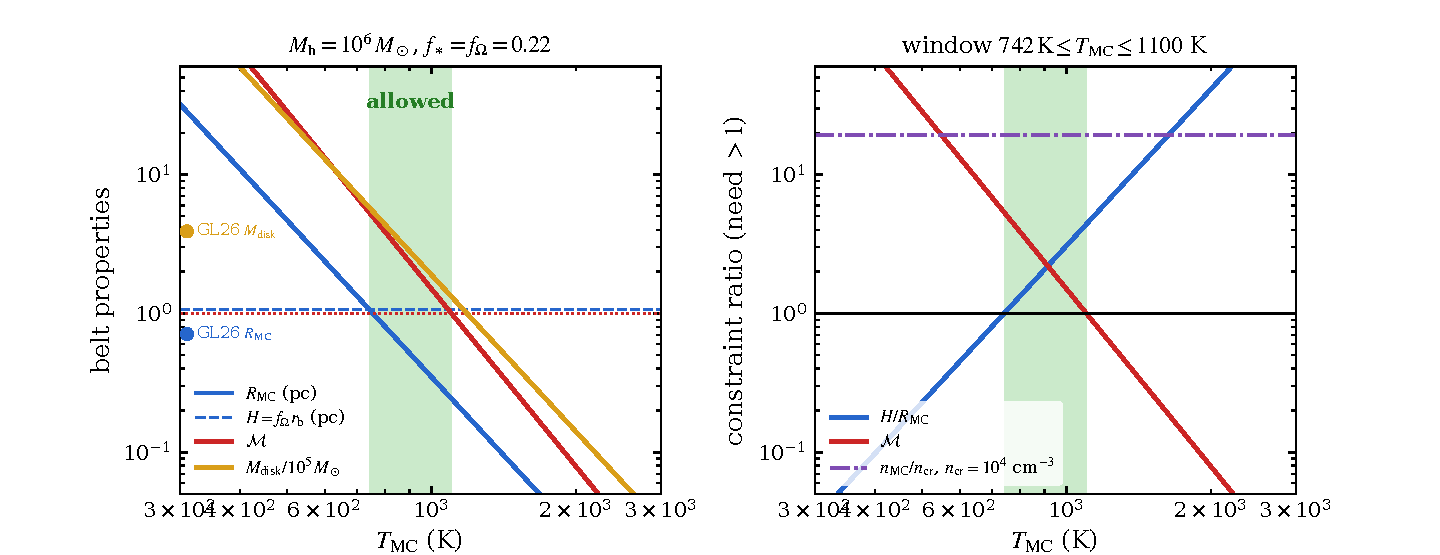
\includegraphics[width=0.98\textwidth]{twindow.pdf}
\caption{Left: cloud radius, Mach number and disk gas mass of the metal-poor belt as functions of the cloud temperature for $\Mh=10^{6}\,\msun$, $\fst=\fOm=0.22$, $\xhh=\zeta=1$. The dashed line is the disk half-thickness $H=\fOm r_{\rm b}$, which does not depend on temperature; the dotted line marks $\mathcal{M}=1$. The corresponding \GL\ values for the CO-cooled belt at 10~K are marked at the left edge for reference. Right: the two consistency ratios that must exceed unity, $H/R_{\rm MC}$ (clouds fit in the disk) and $\mathcal{M}$ (clouds are supersonically turbulent), together with the ratio of the cloud density to a nominal LTE critical density of $10^{4}$~cm$^{-3}$. The shaded band is the allowed window of equation~(\ref{eq:Twindow}). The temperature of the $\Htwo$-emitting gas is not a free parameter of the model but is confined to a factor of 1.5.}
\label{fig:twindow}
\end{figure*}

The window is narrow enough that the temperature is effectively determined, $T_{\rm MC}\simeq900\,\mhsix^{-0.38}$~K at its geometric center. Whether a single temperature can describe the clouds at all depends on how the energy reaches them, and this needs to be stated. The cooling time of $\Htwo$ gas in the window is short, $t_{\rm cool}\simeq 8\,\Tthree^{-2.8}\xhh^{-1}$~yr, whereas a given cloud of radius $R_{\rm MC}$ is struck by a remnant only every $\tau_{\rm c}(R_{\rm UDR}/R_{\rm MC})^{2}\simeq5\times10^{3}$~yr. Were the energy delivered mechanically at the point of impact, the clouds would be cold almost everywhere and warm only in the $\sim10\,\msun$ each shell sweeps and dissociates \citep{Hollenbach:1980a}, and the sound speed in equations~(\ref{eq:virial}) and (\ref{eq:Tmax}) would be that of the cold bulk rather than of the emitting gas. That is not how the energy arrives. The remnants become radiative at $\sim10^{3}\kms$ (Section~\ref{sec:zeta}) and emit their $1.8\times10^{50}$~erg as $\sim$keV X-rays over a few times $\tau_{\rm rad}\simeq30$~yr, and a new remnant forms every $\Geq^{-1}\simeq70$~yr, so at any moment roughly one is radiating somewhere in the belt. The photoabsorption cross-section of primordial gas at 1~keV, $\sim2\times10^{-23}$~cm$^{2}$ per hydrogen nucleus, gives unit optical depth at $N_{\rm H}\simeq5\times10^{22}$~cm$^{-2}$, comparable to the column through the ambient medium (eq.~\ref{eq:NH}) and a tenth of the column through a cloud, so the X-rays are absorbed throughout the cloud volumes rather than at their surfaces, and only the tail above $\sim3$~keV escapes the belt. The clouds are therefore X-ray dissociation regions \citep{Maloney:1996a,Meijerink:2005a,Wolfire:2022a}: heated volumetrically and quasi-continuously by secondary electrons, which deposit a few tens of per cent of the absorbed energy as heat and the rest in ionization and excitation that is itself reradiated \citep{Dalgarno:1999a}, and cooled through $\Htwo$ rotational lines at a few hundred to $10^{3}$~K, which is where such models place dense irradiated gas and where equation~(\ref{eq:Twindow}) places it. Because $\Lambda_{\rm vol}\propto T^{3.76}$, a factor-of-three fluctuation in heating between remnants produces only a $\sim30$ per cent fluctuation in $T_{\rm MC}$, so a single temperature describes the cloud gas to the accuracy of the calculation, and the sound speed in the virial and sonic conditions is that of the same gas that radiates. The X-rays that escape are a prediction, $L_{\rm X}\lesssim10^{40}$~erg~s$^{-1}$ in quiescence, orders of magnitude below the stacked limits on LRDs \citep{Yue:2024a,Ananna:2024a,Maiolino:2025a,Kokubo:2025a}, so the X-ray weakness of the population constrains the flares and not the engine.

At the center of the window and $\Mh = 10^{6}\,\msun$, the belt has $R_{\rm MC} = 0.52$~pc, $\mathcal{M} = 2.4$, $\sigma_{\rm cl} = 4.3\kms$, $M_{\rm MC} = 3.6\times10^{3}\,\msun$, $N_{\rm MC} = 77$, and $M_{\rm disk} = 2.8\times10^{5}\,\msun$ (Table~\ref{tab:compare}). Across the whole window $M_{\rm disk}$ ranges from $1.3\times10^{5}$ to $5.8\times10^{5}\,\msun$, straddling the $3.9\times10^{5}\,\msun$ of the metal-rich solution. That a belt cooled by $\Htwo$ at $\sim10^{3}$~K should so closely resemble one cooled by CO at 10~K is at first surprising, but follows from the numbers: at the belt density, the cooling per hydrogen nucleus of CO at 10~K, $\Lambda_0 n_{\rm MC}\simeq2.5\times10^{-22}$~erg~s$^{-1}$, is within a factor of two of that of $\Htwo$ at $10^{3}$~K, $L_{\rm LTE}/2\simeq5\times10^{-22}$~erg~s$^{-1}$. The two branches of the equilibrium therefore have nearly the same gross structure and differ in the thermodynamic state of the gas: a Mach number of $\sim30$ in cold gas becomes $\sim2$ in warm gas at the same turbulent velocity.

\begin{deluxetable}{lcc}
\tablecaption{The engine at $\Mh=10^{6}\,\msun$, $\fst=\fOm=0.22$\label{tab:compare}}
\tablehead{\colhead{Quantity} & \colhead{Metal-rich (\GL)} & \colhead{Metal-poor (this work)}}
\startdata
Coolant & CO, dust & $\Htwo$ rotational lines \\
$T_{\rm MC}$ (K) & 10 (imposed) & 740--1100 (derived) \\
$\sigma_{\rm eq}$ (km s$^{-1}$) & 240 & 240 \\
$\Geq$ (yr$^{-1}$) & $1.4\times10^{-2}$ & $1.4\times10^{-2}$ \\
$a_{\rm h}$ (pc) & 0.15 & 0.15 \\
$r_{\rm b}$ (pc) & 4.8 & 4.9 \\
$n_{\rm MC}$ (cm$^{-3}$) & $1.9\times10^{5}$ & $1.9\times10^{5}$ \\
$R_{\rm MC}$ (pc) & 0.71 & 0.52 \\
$\mathcal{M}$ & 32 & 2.4 \\
$\sigma_{\rm cl}$ (km s$^{-1}$) & 6.0 & 4.3 \\
$M_{\rm disk}$ ($\msun$) & $3.9\times10^{5}$ & $2.8\times10^{5}$ \\
$N_{\rm MC}$ & 40 & 77 \\
$L_{\rm MC}$ (erg s$^{-1}$) & $8\times10^{40}$ (CO) & $8\times10^{40}$ ($\Htwo$) \\
$n_{\rm bg}$ (cm$^{-3}$) & $7.4\times10^{3}$ & $3.9\times10^{3}$ \\
$N_{\rm H}$ (cm$^{-2}$) & $1.1\times10^{23}$ & $5.9\times10^{22}$ \\
$A_V$ & 50 & $27\,\Zp$ \\
$L_{\rm AGN}/L_{\rm Edd}$ ($f_{\rm B,-3}$) & 0.051 & 0.026 \\
$\langle\dot M_{\rm TDE}\rangle/\dot M_{\rm amb}$ ($f_{\rm B,-3}^{-1}$) & 1.6 & 3.1 \\
$\dot p_{\rm TDE}/\dot p_{\rm AGN}$ & 9.4 & $\gtrsim30$ \\
Mass floor ($\msun$) & $7.3\times10^{5}$ & $7.0\times10^{5}\,\Tthree^{-3.0}$ \\
$t_{\rm gas}$ (yr) & $5.5\times10^{7}$ & $4.0\times10^{7}$ \\
\enddata
\tablecomments{Metal-poor values are evaluated at the center of the temperature window, $T_{\rm MC}=900$~K, with $\xhh=\zeta=1$. Quantities in the upper block are set by the cusp or by the covering condition and do not depend on composition.}
\end{deluxetable}

\subsection{The compression criterion and the mass floor}\label{sec:floor}

The fourth condition of \GL\ asks whether clouds of the derived properties are capable of compressing the cusp to the dispersion the collision cap demands. Replacing equation~(\ref{eq:C3}) with $t_{\rm relax,MC} = t_{\rm relax,\ast}$ and re-solving the monomial system with the $\Htwo$ cooling function gives the largest dispersion the clouds can sustain,
\begin{equation}
\sigma_{\rm comp} = 2.8\times10^{2}\,\mhsix^{0.43}\,\Tthree^{1.19}\,\xhh^{0.32}\,\zeta^{0.05}\kms,
\label{eq:sigcomp}
\end{equation}
to be compared with the \GL\ value of $2.8\times10^{2}\,\mhsix^{0.40}\kms$ ($272\kms$ for the disk-fed geometry). Requiring $\sigma_{\rm comp}\ge\sigma_{\rm eq}$ gives the mass floor
\begin{equation}
\Mh \ge 7.0\times10^{5}\,\Tthree^{-3.0}\,\xhh^{-0.80}\,\zeta^{-0.12}\ \msun,
\label{eq:floor}
\end{equation}
which is $7\times10^{5}\,\msun$ at $\Tthree=1$ and $1.4\times10^{6}\,\msun$ at $\Tthree=0.8$. The metal-poor engine, like the metal-rich one, cannot run around the $\sim10^{4}\,\msun$ seeds that runaway collisions produce \citep{Pacucci:2025a,Inayoshi:2020a}; it switches on only after the seed has grown by two orders of magnitude, and the argument of \GL\ (\S6.1) about the resulting delay carries over. We note that the $\Tthree^{-3}$ dependence pulls in the same direction as the window of equation~(\ref{eq:Twindow}): holes near the floor have $T_{\rm min}\simeq850$~K and a floor of $\sim10^{6}\,\msun$, so the floor for the metal-poor engine is best quoted as $\Mh\gtrsim10^{6}\,\msun$.

\begin{figure*}
\centering
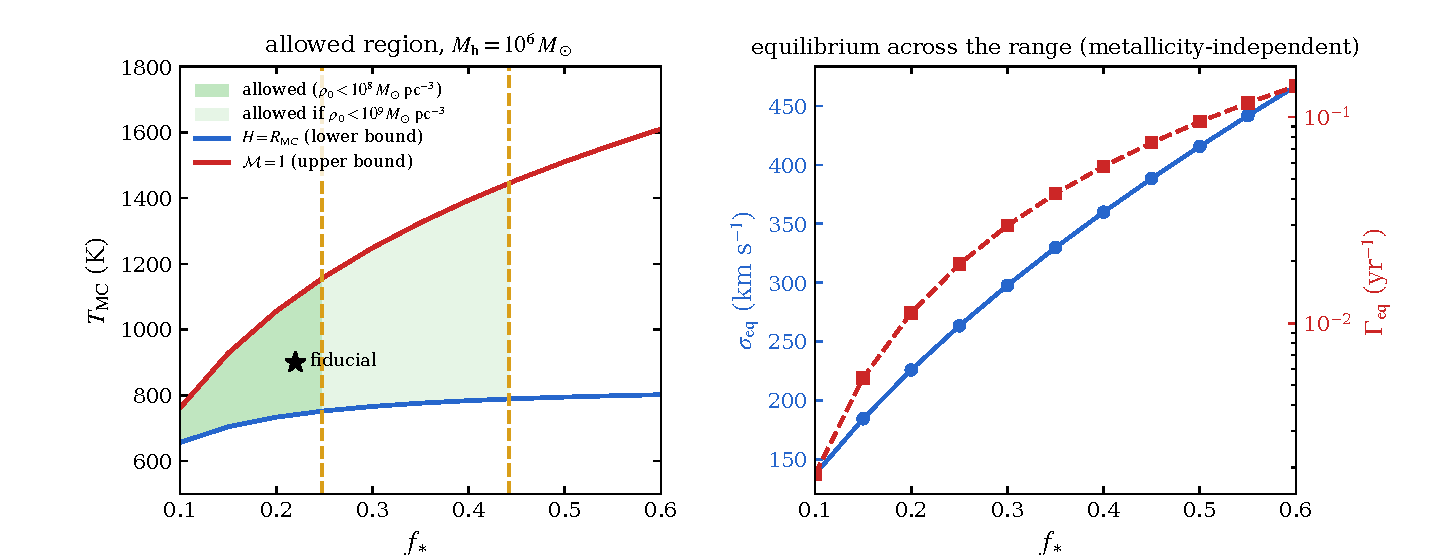
\includegraphics[width=0.98\textwidth]{fplane.pdf}
\caption{Left: the allowed region for the metal-poor engine in the plane of cusp flattening $\fst$ (with $\fOm=\fst$, $b=1$) and cloud temperature, for $\Mh=10^{6}\,\msun$. The lower curve is the geometric requirement $H=R_{\rm MC}$, the upper curve the sonic requirement $\mathcal{M}=1$. The vertical dashed lines mark the flattening at which the cusp central density reaches $10^{8}$ and $10^{9}\,\msun\,{\rm pc^{-3}}$; the darker shading is allowed under the \GL\ ceiling and the lighter shading under the relaxed ceiling appropriate to LRD cores. The AGN-dominance bound of \GL\ does not appear because TDE momentum exceeds AGN radiation pressure everywhere on the plotted range at low metallicity. The star marks the fiducial solution. Right: the equilibrium dispersion and disruption rate across the same range of $\fst$; both are set by the cusp alone and are independent of metallicity.}
\label{fig:fplane}
\end{figure*}

\subsection{The flattening window revisited}\label{sec:fwindow}

\GL\ found that three requirements bound the cusp flattening to $0.18\lesssim\fst\lesssim0.25$: that TDE momentum outweigh AGN radiation pressure ($\fst\gtrsim0.12$), that the clouds fit within the disk ($\fst\gtrsim0.18$), and that the cusp be no denser than observed nuclear star clusters ($\fst\lesssim0.25$ for $\rho_0\le10^{8}\,\msun\,{\rm pc^{-3}}$). Two of the three change character at low metallicity.

The AGN bound disappears. The radiation-pressure coupling in \GL\ is through dust, $\dot p_{\rm rad} = \tau L_{\rm AGN}/c$ with $\tau\simeq30\,f_{\rm Edd}$ for solar dust \citep{Li:2001a,Nenkova:2008b,Netzer:2006a}; in metal-poor gas $\tau\to\max(30f_{\rm Edd}\Zp,\ \tau_{\rm es})$, where the electron-scattering optical depth through the belt is $\tau_{\rm es} = N_{\rm H}\sigma_{\rm T}\simeq0.04$. With $f_{\rm Edd}$ from equation~(\ref{eq:fEdd}) and $\dot p_{\rm TDE} = 1.7\times10^{33}(\Geq/10^{-2}\,{\rm yr^{-1}})$~g~cm~s$^{-2}$ from \GL's equations~(12), (17) and (19), the ratio at $\fst=0.22$ is $\dot p_{\rm TDE}/\dot p_{\rm AGN}\simeq30$ for $\Zp=1$ and $\simeq300$ for $\Zp=0.1$. Tidal disruptions dominate the feedback budget for any flattening the other constraints allow.

The geometric bound is replaced by the pair of temperature bounds. Because $R_{\rm MC}$ now depends on $T_{\rm MC}$, the requirement $H\ge R_{\rm MC}$ is a lower bound on $T_{\rm MC}$ at each $\fst$ (eq.~\ref{eq:Tmin}) rather than a bound on $\fst$ alone, and the sonic requirement $\mathcal{M}\ge1$ supplies the upper bound (eq.~\ref{eq:Tmax}). Repeating the collision-cap and belt solve across $0.10\le\fst\le0.60$ gives the allowed region in the $(\fst,T_{\rm MC})$ plane shown in Figure~\ref{fig:fplane}. It is a wedge that widens toward rounder cusps: at $\fst = 0.10$ the window is $660$--$760$~K, at $0.22$ it is $740$--$1100$~K, and at $0.40$ it is $780$--$1400$~K. The density ceiling is unchanged, since $\rho_0$ depends only on the cusp: $\fst\le0.25\,\mhsix^{0.45}$ for $\rho_0\le10^{8}\,\msun\,{\rm pc^{-3}}$, or $\fst\le0.44\,\mhsix^{0.45}$ if the ceiling is relaxed to the $\sim10^{9}\,\msun\,{\rm pc^{-3}}$ inferred for the most extreme LRD cores \citep{Pacucci:2025a}. The fiducial $\fst = 0.22$ sits inside the allowed region for either choice.

\subsection{The mass range of the metal-poor engine}\label{sec:massrange}

Three considerations confine the metal-poor engine to a narrow range of black hole mass. The floor of equation~(\ref{eq:floor}) is $\sim10^{6}\,\msun$. The LTE treatment of the $\Htwo$ cooling requires $n_{\rm MC}\gtrsim n_{\rm cr}$, where $n_{\rm cr}\sim10^{4}$~cm$^{-3}$ for collisions with H and $\sim10^{5}$~cm$^{-3}$ for collisions with $\Htwo$ (Section~\ref{sec:h2cool}); with $n_{\rm MC}\propto\mhsix^{-2}$ (eq.~\ref{eq:nMC}) this holds for $\mhsix\lesssim1.5$--5 depending on the collider, beyond which the cooling per molecule is suppressed by $(1+n_{\rm cr}/n_{\rm MC})^{-1}$, which acts like a reduced $\xhh$ and pushes the temperature window (eqs.~\ref{eq:Tmin}--\ref{eq:Tmax}) upward. And the gravitational focusing that sets the collision rate requires $\sigma_{\rm h}<v_{\rm esc,\ast}$, which \GL\ show fails above $\sim10^{8}\,\msun$. The binding constraints are the first two, so the metal-poor engine operates for
\begin{equation}
10^{6}\ \lesssim\ \Mh\ \lesssim\ (1.5\mbox{--}5)\times10^{6}\ \msun,
\end{equation}
with disruption rates of $\Geq\simeq(0.5$--$2)\times10^{-2}$~yr$^{-1}$ and cloud temperatures of $400$--$1100$~K across the range. This is the low end of the $10^{6}$--$10^{9}\,\msun$ black hole masses inferred for LRDs from virial estimates on their broad Balmer lines \citep{Harikane:2023a,Matthee:2024a,Greene:2024a}. Those estimates may be biased high: if the line wings are produced by electron scattering rather than Doppler motion, as the highest-quality spectra suggest, the intrinsic line cores imply masses of $10^{5}$--$10^{7}\,\msun$ \citep{Rusakov:2026a}, which brackets the engine's range.

\section{Consequences for little red dots}\label{sec:lrd}

\subsection{Obscuration}\label{sec:obsc}

The most robust prediction of the metal-rich engine was $A_V\simeq50$ through the gas, independent of geometry, and \GL\ identified it as the principal obstacle to an LRD application. It falls away at low metallicity for two reasons. The column itself is lower, $N_{\rm H}\simeq6\times10^{22}$~cm$^{-2}$ at the window center (eq.~\ref{eq:NH}, Table~\ref{tab:compare}), because warm clouds at Mach 2 exert less pressure on the ambient medium than cold clouds at Mach 30 and the ambient density is correspondingly lower. And the dust-to-gas ratio scales with $\Zp$. Together,
\begin{align}
A_V &\simeq 12\,\Zp\,\mhsix^{-4.0}\,\Tthree^{-7.5}\,\xhh^{-2}\,\zeta^{-0.29} \nonumber\\
&\simeq 27\,\Zp\qquad(\Tthree=0.9,\ \mhsix=1),
\label{eq:AV}
\end{align}
so that a nucleus at $\Zp = 0.1$ is seen through $A_V\simeq2.7$ even along sightlines through the disk, and at $\Zp=0.01$ is effectively unobscured. The reprocessed infrared emission is small for a different reason, one that does not scale with $\Zp$ once $A_V\gtrsim1$. The belt intercepts a fraction $\sim\fOm$ of the sky of the hole and absorbs what it intercepts whenever $A_V\gtrsim1$, but it is 30 light-years across, so its dust responds not to the flare being observed but to the luminosity averaged over the duty cycle of Section~\ref{sec:duty}, $\langle L\rangle\simeq F_{\rm Edd}L_{\rm Edd}+L_{\rm AGN}\simeq8\times10^{42}\,\mhsix$~erg~s$^{-1}$. Dust at $r_{\rm b}$ then sits at $T_{\rm d}\simeq60$~K and radiates $L_{\rm IR}\lesssim\fOm\langle L\rangle\simeq2\times10^{42}$~erg~s$^{-1}$ at rest-frame $\sim50$~$\mu$m, about one per cent of the flare luminosity. This is far below the hot-dust limits from MIRI, which probe dust at $\gtrsim300$~K within a fraction of a parsec \citep{Setton:2025a,Chen:2025a}, and the $\lesssim3\times10^{3}\,\Zp\,\msun$ of dust in the belt is three orders of magnitude below the cold-dust limits from ALMA \citep{Casey:2025a}. The dust deficit of LRDs is therefore not in tension with a metal-poor engine; it is what a metal-poor engine predicts.

The gas column is a different matter. $N_{\rm H}\sim10^{23}$~cm$^{-2}$ through the belt at $\sim5$~pc, in gas at $n\sim10^{3}$--$10^{5}$~cm$^{-3}$ and $\sim10^{3}$~K, is not the $N_{\rm H}\gtrsim10^{24}$~cm$^{-2}$ of much denser gas at $\sim10^{3}$ gravitational radii that the ``black hole star'' interpretation requires to produce a Balmer break by gas absorption \citep{Naidu:2025a}. The engine does not itself construct that envelope, though a nucleus in which a $10^{6}\,\msun$ hole is fed intermittently at super-Eddington rates by disruptions, with $\sim3\times10^{5}\,\msun$ of gas within a few parsecs, is not an implausible place for one to form.

\subsection{Luminosity and duty cycle}\label{sec:duty}

The engine does not power an LRD continuously. The Bondi-fed luminosity of equation~(\ref{eq:fEdd}) is $\sim3\times10^{-2}f_{\rm B,-3}L_{\rm Edd}\simeq3\times10^{42}\,\mhsix$~erg~s$^{-1}$, two orders of magnitude below the bolometric luminosities of $10^{44}$--$10^{45}$~erg~s$^{-1}$ inferred for LRDs. What the engine supplies is a high rate of flares. Following \GL's equation~(13), the fraction of time the hole spends above its Eddington luminosity from disruption fallback is $F_{\rm Edd} = 1.3\times10^{-2}\,\mhsix^{-0.4}\,\Gamma_{-2}\simeq1.9\times10^{-2}\,\mhsix^{-1.24}$, and the fraction above $0.1\,L_{\rm Edd}$ is about four times larger for a $t^{-5/3}$ decay, $F_{0.1}\simeq7\times10^{-2}\,\mhsix^{-1.24}$, provided the peak fallback rate exceeds Eddington, as it does for $\Mh\lesssim10^{7}\,\msun$, and the duration is set by the decaying tail rather than the rise. An engine nucleus is therefore observed as a bright, broad-lined source $\sim2$--7 per cent of the time, at luminosities near and above $L_{\rm Edd}\simeq1.3\times10^{44}\,\mhsix$~erg~s$^{-1}$.

This bears directly on the abundance argument. \citet{Bellovary:2025a} noted that a per-system rate of $\sim10^{-4}$~yr$^{-1}$, equivalent to a duty cycle of $\sim10^{-4}$ for year-long flares, is needed to reconcile the observed LRD density with the predicted abundance of runaway-collapse clusters, and that this requirement is in tension with the halo mass function unless the initial mass function is top-heavy. With a duty cycle of $\sim7\times10^{-2}$ instead, the required density of engine hosts is
\begin{equation}
n_{\rm host}\simeq\frac{n_{\rm LRD}}{F_{0.1}}\simeq\frac{10^{-5}\ {\rm cMpc^{-3}}}{7\times10^{-2}}\simeq 1.4\times10^{-4}\ {\rm cMpc^{-3}},
\end{equation}
using the spectroscopic LRD number density of \citet{Matthee:2024a}; the photometric censuses give values up to an order of magnitude higher \citep{Kokorev:2024a,Akins:2025a}, and $n_{\rm host}$ scales with them. This is nearly three orders of magnitude fewer hosts than the low-rate picture requires, and comparable to the abundance of halos of a few$\,\times10^{11}\,\msun$ at $z\sim5$ \citep{Sheth:1999a}, which relaxes the tension without appeal to the initial mass function. \GL\ made the same point qualitatively; the metal-poor solution makes it quantitative for the environment in question.

The same duty cycle makes a prediction about variability. Above $L_{\rm Edd}$ the luminosity is capped near Eddington while the fallback rate is not, so the brightest $\sim2$ per cent of the time is a plateau with little variation; the remaining $\sim5$ per cent, between $0.1$ and $1\,L_{\rm Edd}$, declines as $t^{-5/3}$ over a few years, and a rest-frame baseline of $\Delta t\simeq0.3$--0.5~yr, typical of the multi-epoch JWST imaging at $z\sim5$, samples a change of $(5/3)\Delta t/t\simeq20$--40 per cent at $t\simeq2$~yr. Existing studies find no variability in most LRDs, at limits of a few tenths of a magnitude, and a minority of strongly variable candidates \citep{Kokubo:2025a,Tee:2025a,Zhang:2025a}. Simulated light curves show that super-Eddington disks reproduce that absence where sub-Eddington AGN variability models do not, and that the ongoing high-cadence JWST campaigns will detect continuum changes of $\Delta m>1$ only for the lowest-mass sources \citep{Secunda:2026a}; the Eddington-capped plateau of the engine sits on the same side of that comparison. Roughly a quarter of engine LRDs would be caught on the plateau and the rest in the tail, at the level those limits are beginning to probe, so the population statistics are a marginal test now and a sharp one with longer baselines. Two effects would soften the tail further: the electron-scattering envelope invoked to explain the line wings \citep{Rusakov:2026a} smooths and delays the variations, and the $2\Mh$ of stars inside $a_{\rm h}$ flattens the fallback below $t^{-5/3}$ at late times \citep{Ona:2025a}. What is firm is the repetition: an engine nucleus produces a fresh flare every $\Geq^{-1}\simeq70\,\mhsix^{0.84}$~yr, so an LRD that has faded should rebrighten within a human lifetime.

\subsection{Black hole growth}\label{sec:growth}

Equation~(\ref{eq:mdotratio}) gives $\langle\dot M_{\rm TDE}\rangle/\dot M_{\rm amb}\simeq3\,f_{\rm B,-3}^{-1}$ at the window center, compared with $1.6$ in the metal-rich disk-fed solution. The lower ambient density of the warm belt tips the balance toward the disrupted stars, and for any Bondi efficiency below $3\times10^{-3}$ the hole grows predominantly in the ``black tide'' mode of \citet{Young:1977a}; $N$-body models of dense nuclear clusters around $10^{3}$--$10^{5}\,\msun$ holes find the same stellar feeding channel dominant \citep{Kritos:2026b,Wang:2026b}. Over the gas-limited lifetime $t_{\rm gas} = M_{\rm disk}/m_\ast\Geq = 4\times10^{7}\,\mhsix^{0.33}\,\Tthree^{-3.76}\xhh^{-1}$~yr the hole consumes $\sim2\times10^{5}\,\msun$ in stellar material, of order 20 per cent of its mass, in discrete super-Eddington episodes. If the disk is replenished from the host, the ceiling is the cusp consumption time $t_{\rm cusp} = N_\ast/\Geq = 2.8\times10^{8}\,\mhsix^{1.84}$~yr, over which the hole roughly doubles.

\subsection{Warm molecular hydrogen}\label{sec:h2emission}

The energy condition (\ref{eq:C2}) is a statement about where the injected power goes, and in the metal-poor engine it goes into $\Htwo$ rotational lines: $L_{\Htwo}\simeq8\times10^{40}\,\mhsix^{-0.5}$~erg~s$^{-1}$ from $\sim3\times10^{5}\,\msun$ of gas at $\sim10^{3}$~K (eq.~\ref{eq:LH2}). At these temperatures and densities the emission is carried by the pure rotational $0$--$0$~S(0)--S(5) lines at 28.2, 17.0, 12.3, 9.7, 8.0 and 6.9~$\mu$m, with a subdominant contribution from the $1$--$0$ rovibrational lines near 2~$\mu$m. Warm $\Htwo$ radiating dissipated mechanical energy at this level is a known phenomenon: the $\Htwo$-luminous radio galaxies and the intergalactic shock in Stephan's Quintet have $L_{\Htwo}\sim10^{40}$--$10^{42}$~erg~s$^{-1}$ in the rotational lines, excitation temperatures of a few hundred to $10^{3}$~K, and $\Htwo$ emission that exceeds the X-ray and dust emission of the same gas \citep{Appleton:2006a,Ogle:2010a,Guillard:2012a,Lanz:2015a}. The engine belt is a parsec-scale, metal-poor version of the same thing.

No such emission has been reported from an LRD, and we are aware of no published search for it; the only $\Htwo$ emission so far reported at $z\gtrsim7$ is tentative far-ultraviolet fluorescence in stacked spectra of ordinary galaxies \citep{Johnson:2025a}, a different mechanism and gas phase. The reasons are instrumental rather than physical. At $z\sim5$ the rotational lines redshift to $40$--$170$~$\mu$m, beyond the reach of JWST, and the $1$--$0$~S(1) line at 2.12~$\mu$m falls at $\sim13$~$\mu$m, within the MIRI medium-resolution spectrograph but at a predicted flux of a few $\times10^{-20}$~erg~s$^{-1}$~cm$^{-2}$ for the tens of per cent of $L_{\Htwo}$ carried by the vibrational lines---an order of magnitude below what MIRI spectroscopy has achieved on the same line in an AGN host at cosmic noon \citep{Kakkad:2025a}. The $\Htwo$ luminosity is moreover three to four orders of magnitude below the flare luminosity of the LRD itself. The absence of a detection at high redshift therefore carries no information about the model at present.

What the LRD literature does contain is evidence for cool molecular gas of a different kind. Two LRDs at $z\simeq2$ show water-vapour absorption bands at rest-frame $\sim1.4$~$\mu$m, implying a photosphere-like envelope at $T\sim2000$--4000~K \citep{Wang:2026a}, and LRDs identified in the local Universe show Na\,D, K\,{\sc i}, Ca\,{\sc ii} and other low-ionization absorption features characteristic of cool gas envelopes \citep{Lin:2026a}. These are absorption signatures of dense gas at $\gtrsim10^{8}$~cm$^{-3}$ within light-days of the black hole, the envelope invoked by the ``black hole star'' interpretation \citep{Naidu:2025a}, not emission from parsec-scale clouds at $10^{5}$~cm$^{-3}$, and they do not bear on the belt directly. They do establish that molecular gas is present in LRDs and that their nuclei are cooler and denser than those of ordinary broad-line AGN, which is the environment the engine constructs at larger radii.

The prediction is therefore best tested elsewhere. The local LRDs of \citet{Lin:2026a}, at $z\sim0.1$, place the rotational S(1)--S(5) lines and the rovibrational lines within reach of MIRI spectroscopy at fluxes $\sim10^{5}$ times those of their high-redshift counterparts; MIRI has already measured seven $\Htwo$ rotational lines from gas at $n\sim10^{5}$~cm$^{-3}$ in I\,Zw\,18, at 3 per cent of solar metallicity \citep{Hunt:2025a}. Any such object with a black hole of $\sim10^{6}\,\msun$ and a recent starburst is the natural place to look for a compact ($\lesssim10$~pc) reservoir of a few $\times10^{5}\,\msun$ of warm molecular hydrogen at $\sim10^{3}$~K, at Mach 2--4, and without the cold CO-emitting phase that dominates metal-rich nuclei. A detection would fix $T_{\rm MC}$ observationally through the rotational-line excitation temperature, and equation~(\ref{eq:Twindow}) says what value to expect.

\subsection{The molecular fraction}\label{sec:xh2}

The solution requires the belt gas to be predominantly molecular, since $R_{\rm MC}\propto\xhh^{-1}$ and the temperature window shifts as $\xhh^{-1/4}$ (eqs.~\ref{eq:Tmin}--\ref{eq:Tmax}). In truly primordial gas, without dust, $\Htwo$ forms through the H$^{-}$ channel and reaches fractions of only $\xhh\sim10^{-3}$--$10^{-2}$ even behind ionizing shocks \citep{Shapiro:1987a}, since the electrons that catalyse it recombine faster than the molecules form; only above $n\gtrsim10^{8}$~cm$^{-3}$ do three-body reactions convert the gas fully \citep{Palla:1983a}. At $\xhh = 10^{-2}$ the window of equation~(\ref{eq:Twindow}) moves to $2500$--$3300$~K, where $\Htwo$ is collisionally dissociated at $n\sim10^{5}$~cm$^{-3}$, and the $\Htwo$ branch does not exist. The belt is not primordial gas in the dark, however: the X-ray heating of Section~\ref{sec:temperature} maintains an electron fraction of a few $\times10^{-3}$, and the H$^{-}$ channel then forms $\Htwo$ on $\sim5\times10^{4}$~yr regardless of $\Zp$. Whether that channel can drive the gas fully molecular against X-ray dissociation is a question for an XDR chemistry calculation we do not attempt, so we do not rely on it.

The situation is different for even trace metallicity. Grain-catalysed formation proceeds at $\sim3\times10^{-17}\Zp$~cm$^{3}$~s$^{-1}$ per hydrogen nucleus in cold gas \citep{Hollenbach:1979a}, reduced by a factor of $\sim10$ at the $10^{3}$~K gas temperature of the belt because the sticking and formation efficiencies fall with gas temperature \citep{Hollenbach:1979a,Cazaux:2004a}; it converts gas at $n_{\rm MC} = 2\times10^{5}$~cm$^{-3}$ to $\Htwo$ on a timescale $t_{\rm form}\simeq5\times10^{4}\,\Zp^{-1}$~yr, shorter than the crossing time (eq.~\ref{eq:tc}) for $\Zp\gtrsim0.2$ and shorter than the gas-limited engine lifetime $t_{\rm gas}$ (Section~\ref{sec:growth}) for $\Zp\gtrsim10^{-3}$. Since each UDR dissociates only the $\sim10\,\msun$ it sweeps, a small fraction of a $\sim10^{3}\,\msun$ cloud, and since the Lyman--Werner radiation from the nucleus is self-shielded at the $N_{\Htwo}\gtrsim10^{22}$~cm$^{-2}$ columns of the clouds \citep{Draine:1996a,Wolcott-Green:2011a}, gas that arrives in the belt molecular stays molecular, and gas that arrives atomic becomes molecular within the lifetime of the belt for $\Zp\gtrsim10^{-3}$. At the other end, the metal fine-structure lines reach $\sim15$ per cent of the $\Htwo$ cooling at $\Zp\simeq0.3$ (Section~\ref{sec:h2cool}), and by $\Zp\simeq0.7$ the cold CO branch fits within the disk again (Section~\ref{sec:coldbranch}); between the two the belt would settle at a few hundred K with mixed cooling, an intermediate state we have not solved. We therefore regard $\xhh\simeq1$ and pure $\Htwo$ cooling as appropriate for $10^{-3}\lesssim\Zp\lesssim0.3$. This is the metal-poor engine's regime of validity. It brackets the metallicities at which runaway collisions are expected to build the LRD seeds \citep{Pacucci:2025a,Inayoshi:2020a}, and it contains the measured metallicities of LRD hosts, $\Zp\simeq0.08$ with a spread of 0.6~dex and two objects below $0.013$ \citep{Nikopoulos:2026a}. Below $\Zp\sim10^{-3}$ the belt would have to be cooled by atomic processes---Ly$\alpha$ at $\sim8000$~K, with $\Lambda_{\rm vol}\propto n^{2}$ and a dependence on the ionization fraction that the UDR shocks themselves would set---and that branch, if it exists, would need a separate treatment.

\section{Caveats}\label{sec:caveats}

The treatment inherits every simplification of \GL, and \S6.5 of that paper applies without change: the loss-cone rate sits near $q\sim1$ and requires the bridged flux; the normalization of $\Geq$ is uncertain by two orders of magnitude through the collision coefficient $\Lambda_{\rm c}$ while its mass exponent is stable; the compression criterion rests on a plausibility argument rather than a computed torque; and the clouds are treated as a single population at a single radius. To these we add the following.

The cooling function of equation~(\ref{eq:LLTE}) is the rotational LTE rate alone. Including the sub-thermal vibrational contribution at $n\sim10^{5}$~cm$^{-3}$ would raise the cooling per molecule by tens of per cent and steepen its temperature dependence somewhat, shrinking $R_{\rm MC}$ and $M_{\rm disk}$ by the same factor; both effects are within the factor-of-two spirit of the calculation and are absorbed into $\xhh$.

The temperature window is bounded by two conditions of different character. The lower bound, $H\ge R_{\rm MC}$, is the same geometric requirement \GL\ use and is secure. The upper bound, $\mathcal{M}\ge1$, marks where the framework ceases to apply rather than where a solution ceases to exist: a belt of thermally supported clouds at $\sim1500$~K is a self-consistent configuration, but not one in which UDR momentum sustains turbulent support against star formation, which is the mechanism the engine rests on. A treatment of the transition from turbulent to thermal support would be needed to say what happens at the upper edge.

We have assumed the belt gas is fully molecular and argued that dust-catalysed formation makes this so for $\Zp\gtrsim10^{-3}$. The argument uses the grain formation rate of solar-neighbourhood dust scaled linearly with $\Zp$; if the dust-to-gas ratio falls faster than linearly at low metallicity, as observations of dwarf galaxies below $\Zp\sim0.1$ suggest \citep{Remy-Ruyer:2014a,Galliano:2018a}, the lower edge of the validity range moves up accordingly.

Finally, the energy budget of equation~(\ref{eq:C2}) assigns the full UDR luminosity to the clouds, as \GL\ do. In the picture of Section~\ref{sec:temperature} that energy arrives as X-rays, and whatever escapes the belt above $\sim3$~keV, or is deposited in the ambient medium rather than in the clouds, is lost to the budget. We estimate the loss at tens of per cent, comparable to the other uncertainties absorbed into $\xhh$; the escaping part is a prediction rather than a defect. A calculation of the X-ray transfer and XDR chemistry of the belt, which would fix the heating efficiency, the escaping spectrum and the molecular fraction together, is the natural next step.

\section{Summary}\label{sec:summary}

We have re-derived the self-sustaining tidal disruption engine of \citet{Guillochon:2026a} with the cooling function appropriate to metal-poor gas, in which the CO and dust that hold the metal-rich belt at 10~K are absent and the clouds cool instead through $\Htwo$ rotational lines in LTE. Our conclusions are these.

\begin{enumerate}
\item The equilibrium disruption rate, stellar dispersion, cusp density, belt radius and cloud density are independent of composition, because the collision cap involves only the cusp and the covering condition fixes the belt radius without reference to the cooling. $\Geq\simeq1.4\times10^{-2}\,\mhsix^{-0.84}$~yr$^{-1}$, $r_{\rm b}\simeq4.9\,\mhsix$~pc and $n_{\rm MC}\simeq1.9\times10^{5}\,\mhsix^{-2}$~cm$^{-3}$ carry over from \GL\ unchanged.
\item The cold branch of the equilibrium does not exist at low metallicity: with $\Lambda_0\propto\Zp$ the clouds outgrow the disk for $\Zp\lesssim0.7$, and the 10~K thermostat is gone in any case. The engine relocates to a warm branch in which the clouds are heated throughout their volume by the keV emission of the radiative remnants, one of which is radiating in the belt at any moment, and in which the temperature of the $\Htwo$-emitting gas is not imposed but bracketed, by the requirements that the clouds fit within the disk and remain supersonically turbulent, to $740\,\mhsix^{-0.40}\lesssim T_{\rm MC}\lesssim1100\,\mhsix^{-0.36}$~K.
\item Within that window the warm belt has nearly the same cloud radii, gas mass ($\sim3\times10^{5}\,\msun$) and mass floor ($\sim10^{6}\,\msun$) as the metal-rich belt, because $\Htwo$ at $10^{3}$~K and CO at 10~K happen to radiate comparably per hydrogen nucleus at the belt density. What differs is the state of the gas: Mach 2 rather than Mach 30.
\item The observable consequences differ sharply. The extinction is $A_V\simeq27\,\Zp$ rather than 50, and the belt dust, which sees only the duty-cycle-averaged luminosity, reradiates $\sim1$ per cent of the flare luminosity at $\sim60$~K, so the dust deficit of LRDs is expected rather than problematic. The flares recur every $\sim70$~yr and, outside their Eddington-capped plateau, decline by tens of per cent over rest-frame half-year baselines. AGN radiation pressure is negligible, so the lower bound on the cusp flattening moves from feedback dominance to the sonic condition, and the allowed region in the $(\fst,T_{\rm MC})$ plane is a wedge that widens toward rounder cusps. The black hole grows predominantly through disruptions. The injected energy emerges as warm $\Htwo$ emission at $L_{\Htwo}\simeq8\times10^{40}\,\mhsix^{-0.5}$~erg~s$^{-1}$.
\item The metal-poor engine operates for $10^{6}\lesssim\Mh\lesssim(1.5$--$5)\times10^{6}\,\msun$, bounded below by the compression criterion and above by the LTE requirement on the $\Htwo$ cooling, and for $10^{-3}\lesssim\Zp\lesssim0.3$, bounded below by the need for dust-catalysed $\Htwo$ formation within the belt lifetime and above by the point at which metal fine-structure cooling becomes competitive, with the cold CO branch returning at $\Zp\gtrsim0.7$. The range contains the measured metallicities of LRD hosts. Above a tenth of the Eddington luminosity $\sim7$ per cent of the time, it requires an LRD host abundance of $\sim10^{-4}$~cMpc$^{-3}$, nearly three orders of magnitude fewer hosts than a $10^{-4}$~yr$^{-1}$ rate would need.
\end{enumerate}

The picture that emerges is of a nucleus that has just finished building a $\sim10^{4}\,\msun$ seed by runaway collisions in metal-poor gas, grows it by accretion to $\sim10^{6}\,\msun$, and then enters a collisionally regulated state in which it disrupts a star every century, is seen as an LRD a few per cent of the time, and is surrounded not by the cold, dusty, CO-bright molecular disk of a metal-rich engine but by a few $\times10^{5}\,\msun$ of warm, dust-poor molecular hydrogen at a thousand kelvin.

\begin{acknowledgments}
The manuscript source, the bibliography, and the equilibrium-solver and figure scripts are available online.\footnote{\url{https://github.com/guillochon/engine-lrds}} The authors take full responsibility for the contents of this paper. Large language models (Claude Fable 5.1, Grok 4.6, and GPT5.6 Sol) were used, under author supervision, to draft and edit the text, to derive and check analytic results, to write and refine the analysis and figure-generation scripts released with this paper, and to refine the presentation of the figures. The figures themselves are produced by those scripts from the solver outputs; no generative model created or altered the plotted data. Every displayed equation has been re-derived independently, every entry in the bibliography was validated against the NASA Astrophysics Data System, and all references and AI edits were hand-checked by the authors. We aimed to be compliant with the AAS guidelines on generative AI in manuscript preparation.\footnote{\url{https://journals.aas.org/author-llm-guidelines}} Those guidelines do not treat such tools as authors; responsibility for accuracy remains with the listed authors. We thank J. Xavier Prochaska for providing access to AI models that were used to conduct independent AI reviews.
\end{acknowledgments}

\software{\texttt{numpy}, \texttt{scipy}, \texttt{sympy}, \texttt{matplotlib}; the \texttt{tde-engine} scripts of \GL.}

\bibliographystyle{aasjournal}
\bibliography{lrd}

\end{document}
